\begin{figure}[t]
\centering
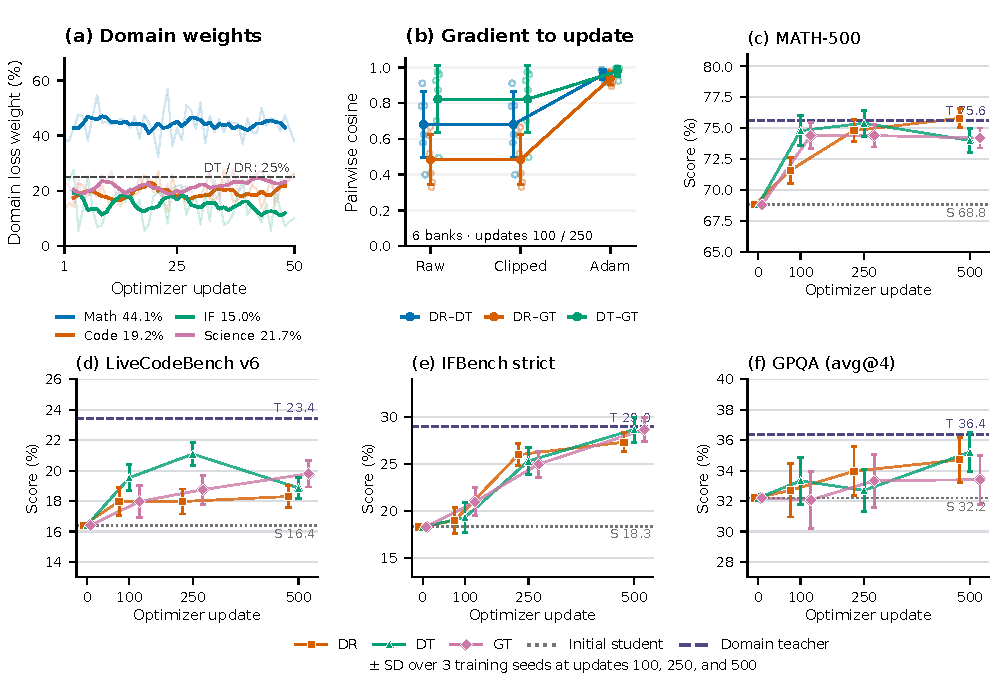
\includegraphics[width=\linewidth]{figures/table1_sync_20260918/section3_normalization.pdf}
\caption{\textbf{Loss averaging changes gradient directions; Adam produces more aligned updates and similar final mean scores.}
(a) Domain shares under global token averaging (GT).
(b) Gradient and update cosines for global token, within-domain token (DT), and within-domain response (DR) averaging; points and bars show batch means and standard deviations.
(c--f) Task learning curves under top-64 intersection supervision (I64); S/T mark the initial student/teacher; error bars show model-based question-sampling standard deviations.}
\label{fig:normalization_capability}
\end{figure}
